\section{Mining Process}

\subsection{Clustering}

\begin{wrapfigure}{r}{0.4\textwidth}
\vspace{-0.5cm}
  \begin{center}
    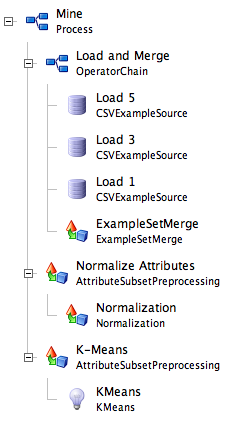
\includegraphics[scale=0.5]{images/mine.png}
  \end{center}
  \caption{Mine Process}
  \label{figure:mine}
\end{wrapfigure}


Since all the data coming from the preprocessing are unlabeled, we chose an unsupervised learning approach for our mining process (shown in Figure \ref{figure:mine}); so we start with a clustering operation on all the data.

After the preprocessing step we have a distinct file for each car involved in the test, so we have to merge all of them. 

Once all the data are stored in a single location, we can normalize the numerical attributes \texttt{Speed} and \texttt{EngineSpeed}, in order to make them weight the same during the clustering process.

Finally the clusters are computed, using the k-means algorithm with 3 centroids; this number of final clusters seemed to provide the better result.
\newline


Figure \ref{figure:clusters} shows the cluster distribution with respect to the \texttt{Speed} and\newline \texttt{EngineSpeed} attributes.

\begin{figure}[h!]
\centerline{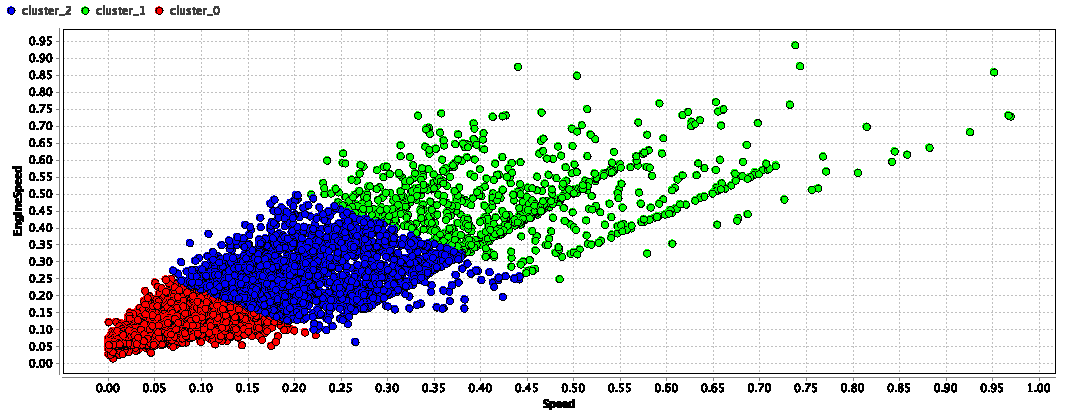
\includegraphics[width=\textwidth]{images/cluster_distrib.png}}
\caption{Clustering result}
\label{figure:clusters}
\end{figure}

